\begin{figure}
 \centering
% 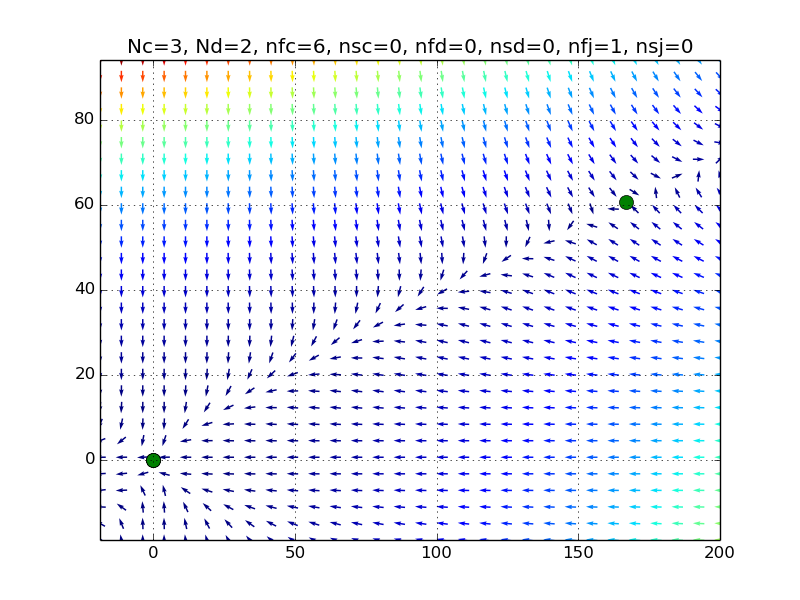
\includegraphics[scale = 0.5]{abschnitte/beta_QCDxdQCD/fig/RG_flow3_2_6_0_0_0_1_0.png}
% 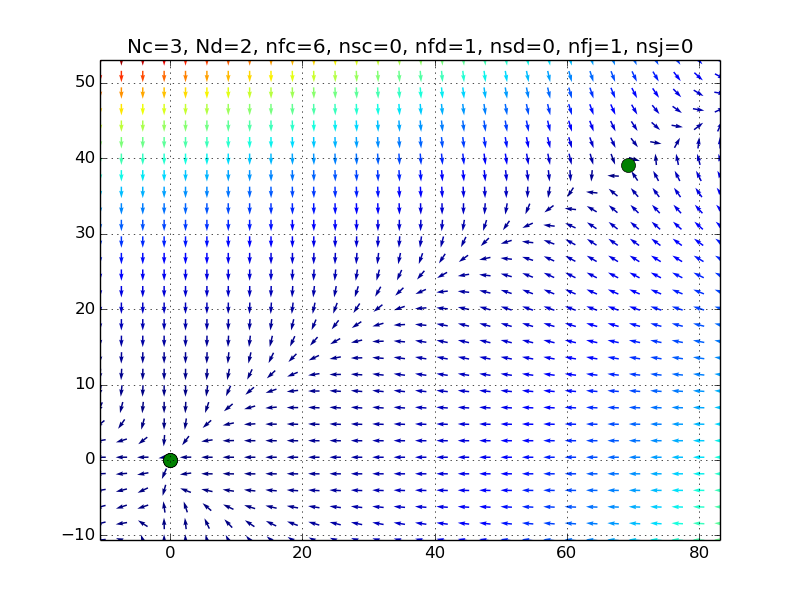
\includegraphics[scale = 0.5]{abschnitte/beta_QCDxdQCD/fig/RG_flow3_2_6_0_1_0_1_0.png}
 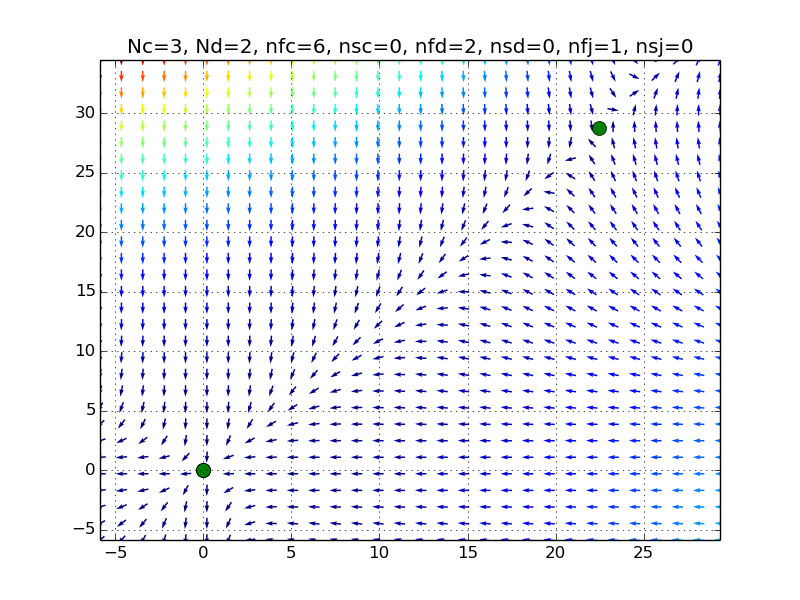
\includegraphics[scale = 0.5]{abschnitte/beta_QCDxdQCD/fig/RG_flow3_2_6_0_2_0_1_0.png}
 \caption{Flussdiagramm für den Sattelpunkt $\alpha^{*4}$.}
 \label{fig:beta_QCDxdQCD:Sattelpunkt1}
\end{figure}
